\subsubsection{Raspberry Pi}
\begin{figure}[H]
  \centering
  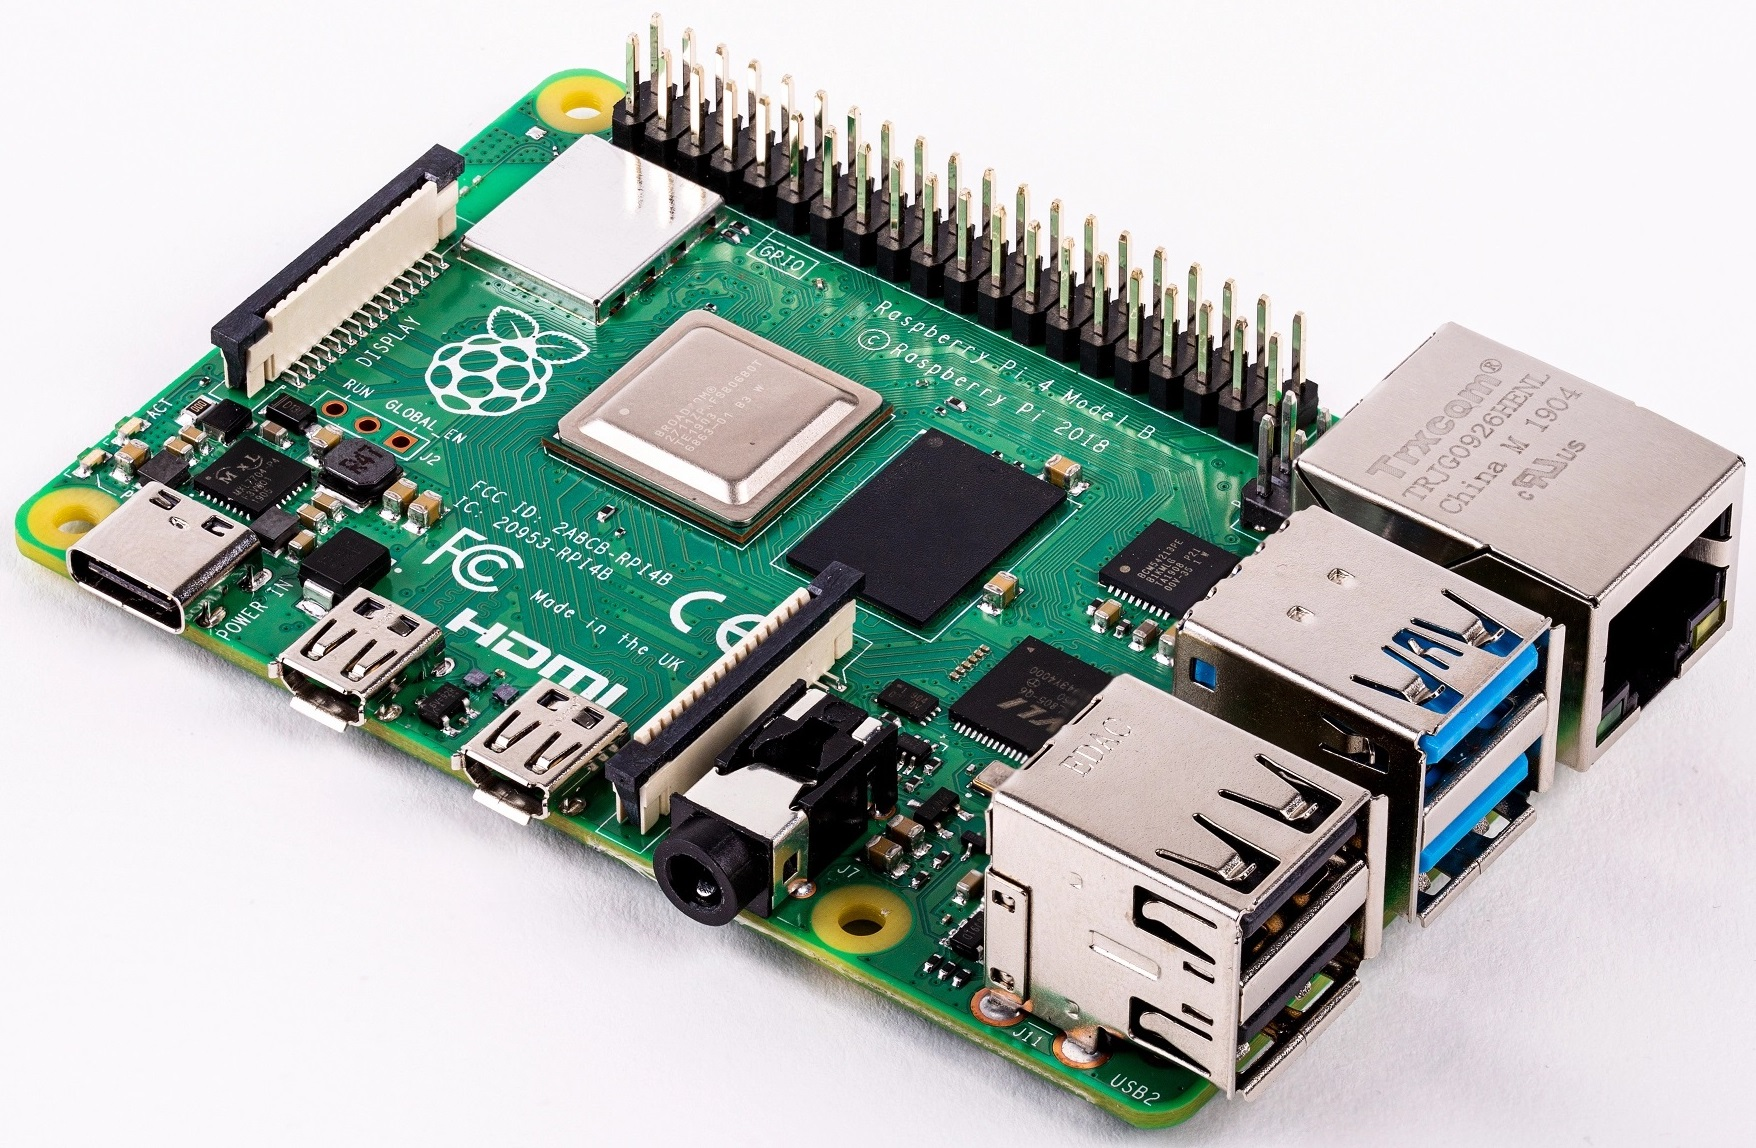
\includegraphics[width=4cm]{images/techAnalysis/Pi4B.jpg}
  \caption{Raspberry Pi 4B \cite{RaspberryPI-figure-Pi4b}}\label{fig:sssec:raspberrypi-Pi4B}
\end{figure}
Raspberry Pi is a line of small computers which are powerful compared too their price \cite{raspberry_pi_foundation_raspberry_nodate} \cite{raspberry_pi_foundation_what_nodate}.
The first generation of the Pi called model A has a 32-bit processor running at 700MHz, 256MB RAM only a single USB port and no ethernet, WIFI or Bluetooth \cite{raspberry_pi_foundation_raspberry_nodate} \cite{raspberry_pi_foundation_bcm2835_nodate} \cite{arm_limited_arm11_nodate}.
Since the first model, multiple generations have been released with improvements in the hardware specifications.
The newest model is the fourth generation model B, which can be seen in \autoref{fig:sssec:raspberrypi-Pi4B}.
This model has a 64bit ARMv8-A processor running at 1,5GHz and has either 1GB, 2GB or 4GB of RAM.
It also features multiple USB ports, an ethernet port, WIFI, and Bluetooth.
The predecessor to the 4B used the same GPU, but along with other upgrades, the GPU in the 4B is also updated to a more powerful one \cite{raspberry_pi_foundation_raspberry_2019}.
All other versions than the 4B have HDMI connection for video and sound, where the new version of the Raspberry Pi has a newer HDMI standard and two micro-HDMI ports, instead of one normal sized HDMI port as the rest.
The first generations had an RCA composite jack, but this has been replaced by a 3.5mm jack in the subsequent versions.
Beside this, all versions have general-purpose input/output pins, DSI port for raw displays, CSI-2 camera port, storage through SD cards in the old version, and through SDHC cards in the newer versions.
The newer the version are, the more power it consumes, where the old 1B+ under max stress consumes 1.75 watt (0.35amp at 5v), the newer model 4B consumes 6.25 watt (1.25amp at 5v).
\cite{raspberry_pi_foundation_faqs_nodate}

The available Raspberry Pi models for the project is the B+, 2B, 3B, 3B+ and 4B with 4gb RAM.
